Nesse capítulo será apresentado o Linderhof que foi a ferramenta implementada para efetuar o ataque. Iremos detalhar a arquitetura, funcionalidades e como adicionar novos ataques ao Linderhof. A ferramenta tem o objetivo para facilitar o desenvolvimento de ataques DoS refletidos.

\section{Arquitetura}

A arquitetura do Linderhof foi pensada para ser a mais modular possível. Ela possui 3 módulos como mostra a figura \ref{img:linderhof}, Oryx (interface), Commander e Netuno(injetor de pacotes). Cada \textit{engine} periférica do Linderhof não impacta o módulo Commander, sendo possível utilizar qualquer outra interface e injetor.

\begin{figure}[H]
     \centering
     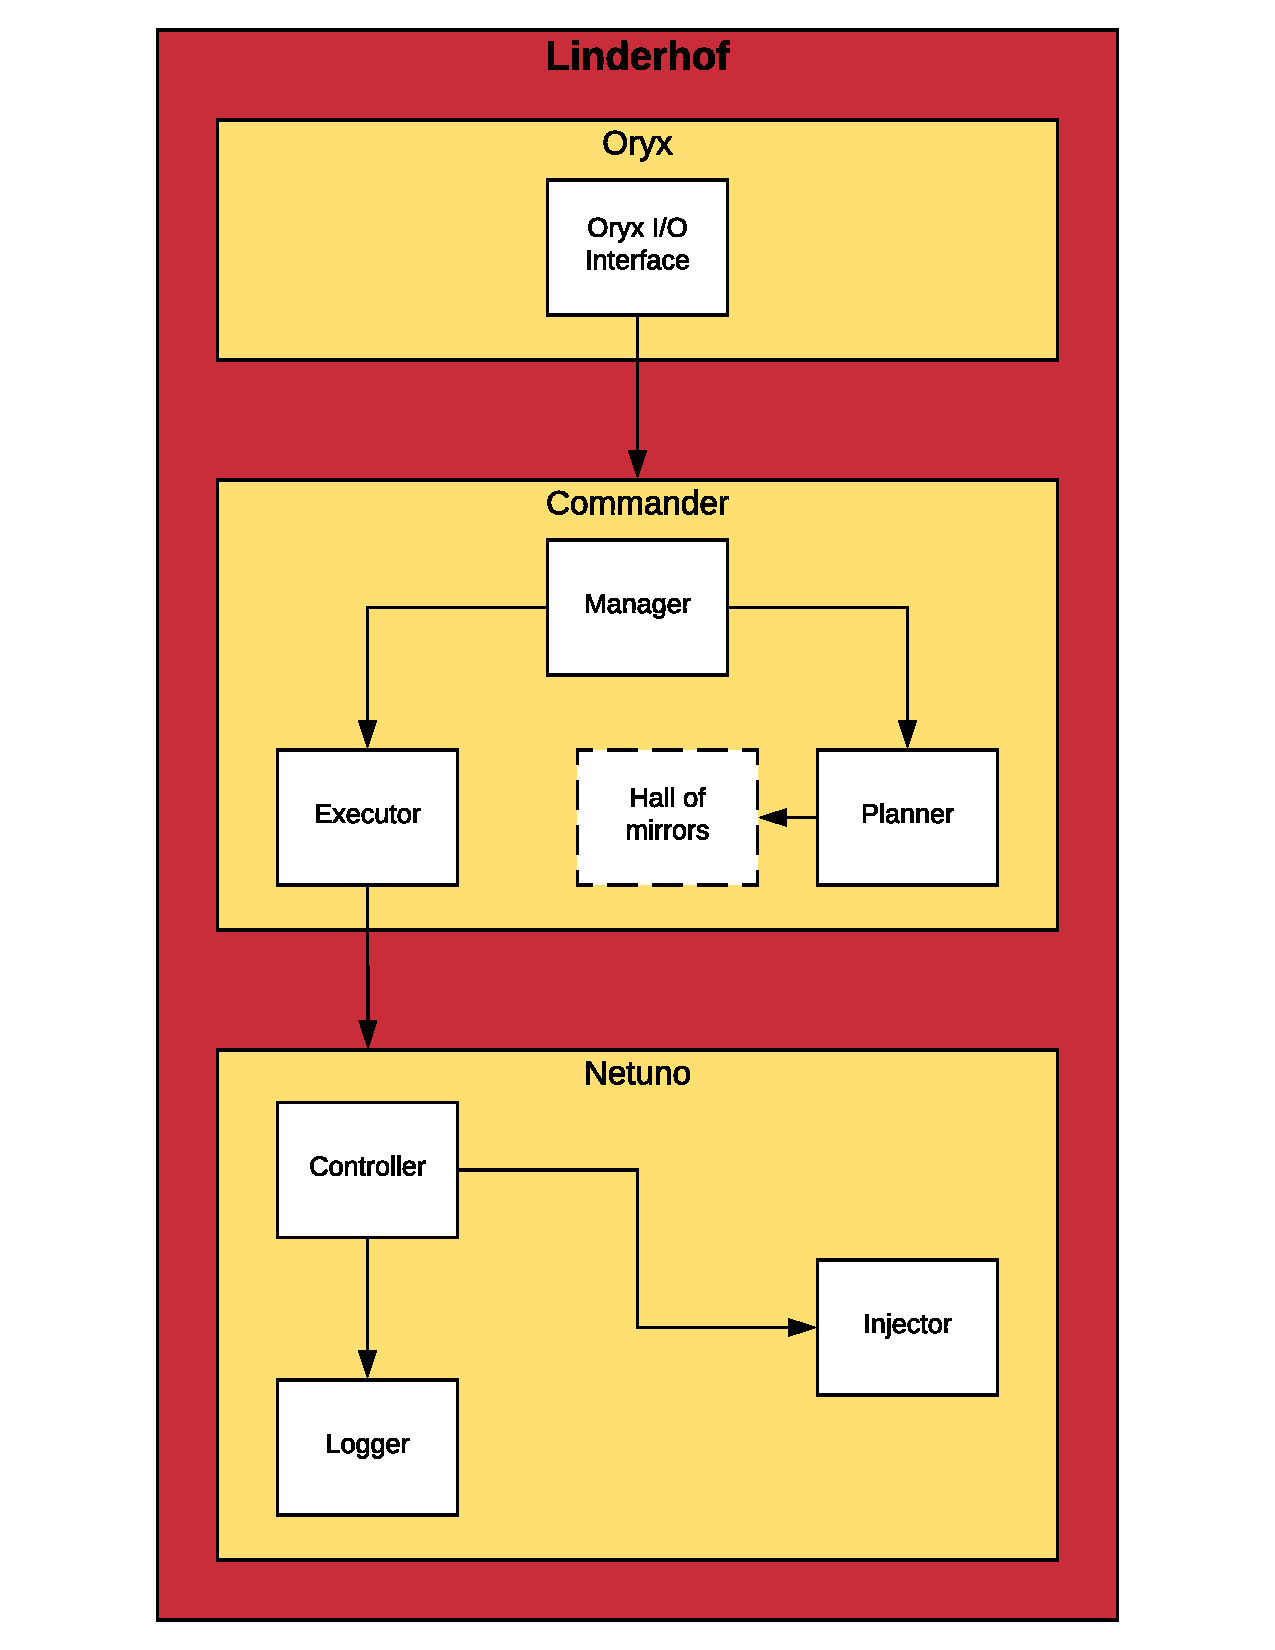
\includegraphics[scale=0.6]{img/Linderhof.pdf}
     \caption{Arquitetura Linderhof }
     \label{img:linderhof}
\end{figure}

\subsection{Módulo Oryx}

O módulo Oryx é a \textit{engine} de interface de usuário do Linderhof. Seu trabalho principal é criar a estrutura de \textit{draft} do ataque que será executada. Os argumentos que podem ser passados para a interface e são apresentados na figura \ref{img:optlhf}. Ao terminar de montar a estrutura \textit{draft} o Módulo Oryx o encaminha para o Módulo Commander.

\begin{figure}[H]
     \centering
     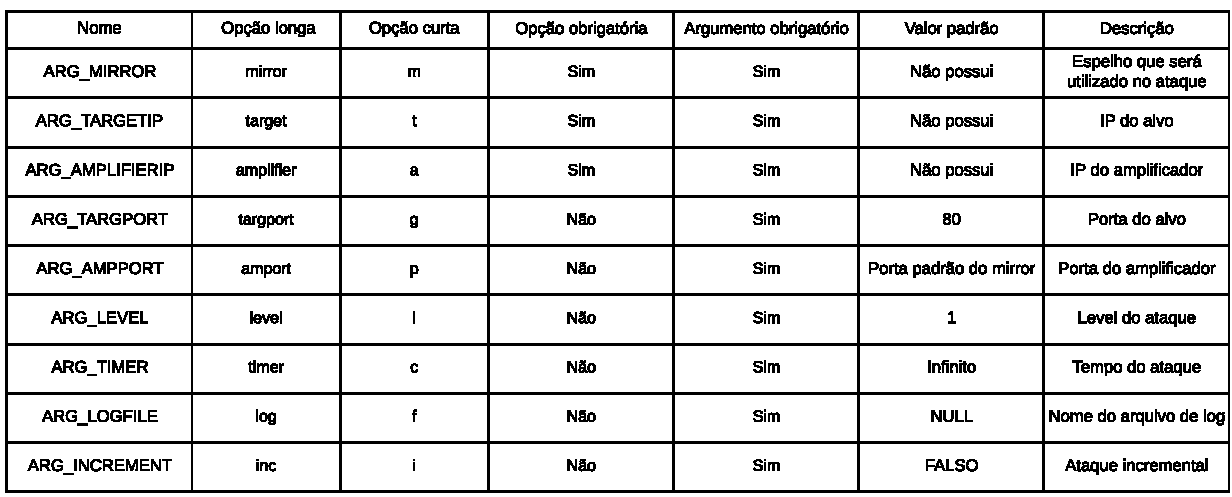
\includegraphics[scale=0.8]{img/Opcoes_lhf.pdf}\
     \caption{Opções da interface Oryx}
     \label{img:optlhf}
\end{figure}


\subsection{Módulo Commander}

O módulo Commander é o núcleo da ferramenta. Ele é responsável por criar o planejamento do ataque de acordo com \ \textit{draft} passado pelo módulo superior e chamar o injetor Netuno com os argumentos necessários para executar o ataque. Esse módulo é subdividido em 4 submódulos: Manager, Planner, Executor e Hall of mirros. 

O Hall of mirros contém as funções de chamada para cada ataque, chamamos essas funções de mirror. Os mirrors tem a finalidade de fazer toda a preparação para o ataque e chamar o injetor para executar o ataque quando tudo estiver preparado. Essa preparação consiste em criar todos os pacotes para o injetor e fazer todo a preparação dos refletores antes do ataque.

O módulo Manager gerencia o Planner e o Executor, funcionando como uma ponte entre eles. Além disso ele tem a responsabilidade de validar o draft recebido e fazer a inicialização da ferramenta como setar os handler de sinal, adicionar as Linux \textit{capabilities} necessárias e funções de error.

O Planner é responsável por montar a estrutura de plano de ataque de acordo com o mirror desejado. Essa estrutura contém o tipo do mirror, a função de chamada do mirror, e os dados necessário para executar a função de chamada do ataque.

O Executor tem a única responsabilidade de executar o mirror.

\subsection{Módulo Netuno}

O módulo Netuno é a engine de injeção do Linderhof. Ele foi implementado para conseguir uma injeção de pacotes constante no ataque. É dividido em 3 submódulos, Controller, Injector e Logger. 

O Injector tem a responsabilidade de criar e destruir as \textit{threads} injetoras. Cada injetor possui um bucket que corresponde a quantidade de pacotes que ele deve enviar.
O Controller é responsável por controlar a taxa de injeção de cada injetor através da atualização do bucket dos injetores de acordo com o intensidade do ataque desejada e encerrar o ataque de acordo com o timer passado pelo usuário. O Netuno tem a opção de executar um ataque incremental, nesse tipo de ataque ele irá aumentar o nível a uma frequência que foi passado pelo usuário. O Logger faz apenas o log do ataque em execução pode ser apresentado no terminal ou salvo em um arquivo.

A intensidade do ataque corresponde a quantidade de pacotes que o Netudo deve enviar por segundo, e essa parâmetro e passado através do argumento nível do Oryx. A quantidade de pacotes por segundo respeita a seguinte fórmula:

\begin{equation}
10^{L - 1}
\label{cal:Fator_Memcached2}
\end{equation}

Onde L corresponde a intensidade do ataque deseja. Resultando na seguinte tabela:

\begin{table}[H]
\centering
\label{tab:pacotes/s}
\caption{Intensidade por pacotes/segundo}
\begin{tabular}{|c|c|}
\hline
\multicolumn{1}{|l|}{\textbf{Level}} & \multicolumn{1}{l|}{\textbf{Pacotes/segundo}} \\ \hline
1                                    & 1                                             \\ \hline
2                                    & 10                                            \\ \hline
3                                    & 100                                           \\ \hline
4                                    & 1000                                          \\ \hline
5                                    & 10000                                         \\ \hline
6                                    & 100000                                        \\ \hline
7                                    & 1000000                                       \\ \hline
8                                    & 10000000                                      \\ \hline
9                                    & 100000000                                     \\ \hline
10                                   & 1000000000                                    \\ \hline
\end{tabular}
\end{table}

É importante ressaltar que esse parâmetro indica o fluxo de pacotes desejado no ataque. Isso não significa que a máquina atacante conseguirá gerar a quantidade de pacotes desejada e nem que a quantidade de pacotes gerados chegará ao amplificador.

\section{Adicionando um novo mirror}

Como dito anteriormente um mirror é responsável por fazer toda a preparação doa ataque como forjar os pacotes para o injetor e fazer a preparação do amplificador para o ataque. Após finalizar a preparação ele deve chamar o injetor para iniciar o ataque.

Para adicionar um novo mirror ao Linderhof devemos fazer algumas pequenas alterações nos módulos Oryx e Controller. A seguir iremos apresentar quias são essa alterações.

\begin{enumerate}
    \item \textbf{Criar função de chamada do mirror}
    
    A função de chamada do mirror deve seguir o protótipo a seguir:
    
    \begin{lstlisting}
    int ExecuteMirrorNameMirror( void * p_arg );
    \end{lstlisting}
    
    Sendo \texttt{p\_arg} os argumentos necessários para executar o mirror. 
    
    Os arquivos do mirror devem ficar na pasta \texttt{src/linderhof/hom/nome\_do\_mirror}.

    A função de chamada será declarada em \texttt{src/linderhof/hom/nome\_do\_mirror.h}.
    
    \item \textbf{Adicionar mirror ao Linderhof planner}
    
        \begin{enumerate}
            \item Adicione seu mirror no enum MirrorType em src/include/venus.h
            \item Atualize o switch-case da função Planner para construir o LhfPlan do seu mirror. O ponteiro atkData deve conter os argumentos que serão utilizados pelo mirror.
        \end{enumerate}
        
    \item \textbf{Adicionar mirror a engine UI Oryx}
    
        Na função src/interface/interface.c:parserAttackOpt adicione a construção do draft do mirror.
\end{enumerate}

\section{Considerações finais}

Nesse capítulo foi apresentado o \textit{design}, funcionamento do Linderhof e como adicionar novos mirrors a ele. De modo geral a ferramenta tem o objetivo para facilitar o desenvolvimento de ataques DoS refletidos, retirando o retrabalho de implementação dos módulos de injeção e interface.

No capítulo \ref{cap:Apresetacao} utilizaremos o Linderhof no papel de atacante para viabilizar a simulação de uma ataque DoS refletido Memcached em laboratório. 
